% Begin the document and set up the style of the document
\documentclass[a4paper]{article}

% Install the required packages for the document 
\usepackage{envmath}
\usepackage{esvect}
\usepackage{graphicx}
\usepackage{gensymb}
\usepackage{tikz}
\usepackage[mathcal]{euscript}
\usepackage{geometry}
\usepackage{enumitem}
\usepackage{mathtools}
\usepackage{subdepth}
\usepackage{graphicx}
\usepackage{amsmath}
\usepackage{amscd}
\usepackage{amssymb}
\usepackage{amsfonts}
\usepackage{harpoon}
\usepackage[title]{appendix}
\usepackage{pgf}
\usepackage{tikz}
\usepackage{mathrsfs}
\usepackage{asyalign}
\usepackage{physics}
\usepackage{enumitem}
\usepackage{xhfill}
\usepackage{accents}
\usepackage{cite}
\usepackage{url}
\usepackage{csquotes}
\usepackage{wrapfig}
\usepackage{booktabs}
\usepackage{adjustbox}
\usepackage{caption}
\usepackage{minipage-marginpar}
\usepackage{calc}
\usepackage[tableposition=top]{caption}
\usepackage{ifthen}
\usepackage[utf8]{inputenc}
\usepackage{tikz-3dplot}
\usetikzlibrary{patterns}
\usetikzlibrary{arrows}

% Page and style settings
\parskip=8pt
\parindent=0pt
% Right margin
\textwidth=6.25in
% Left margin
\oddsidemargin=0pt
\evensidemargin=0pt
% Bottom margin
\textheight=10in
% Top margin
\topmargin=-0.75in
\baselineskip=11pt
% end of page and other style settings

\renewcommand{\familydefault}{\sfdefault}

\newcommand{\indep}{\mathrel{\text{\scalebox{1.07}{$\perp\mkern-10mu\perp$}}}}
\newcommand{\p}{\mathbb{P}}
\newcommand{\e}{\mathbb{E}}
\newcommand{\ds}{\displaystyle}
\newcommand{\code}{\texttt}

% Begin the text of the document
\begin{document}

\newlength{\strutheight}
\settoheight{\strutheight}{\strut}

% Begin the Title Page
\begin{titlepage}

\newcommand{\HRule}{\rule{\linewidth}{0.5mm}} % Defines a new command for the horizontal lines, change thickness here

\center % Center everything on the page
 
\textsc{\LARGE University of New South Wales}\\[1.5cm] % Name of your university/college
\textsc{\Large COMP 2521}\\[0.5cm] % Major heading such as course name
\textsc{\large Data Structures and Algorithms}\\[0.5cm] % Minor heading such as course title

\HRule \\[0.4cm]
{ \huge \bfseries Lab 04 Report}\\[0.4cm] % Title of your document
\HRule \\[1.5cm]


\begin{center} \large
Jack English (z5208352), Keegan Gyoery (z5197058)% Your name
\\
\end{center}


\vspace{4cm}

{\today}\\[3cm] % Date, change the \today to a set date if you want to be precise

\vfill % Fill the rest of the page with whitespace

\end{titlepage}

\pagenumbering{arabic}

\tableofcontents
\listoftables

\pagebreak

\section{Introduction}
The following report details the attempt to determine the algorithms used for two sorting programs, the code of which is unable to be seen. Thus, constructing an experiment to highlight the stability, time taken to complete, and adaptivity of the sorting programs will give insight into the possible algorithms used. Different data sequences will be used based on the properties of each algorithm, and will be tailored to make it as obvious as possible as to which algorithm is in use.

\section{Experimental Design}

\subsection{Correctness Analysis}
Each of the two given sorting programs will be tested through a range of different input sequences, and their output collected. The collected output will be compared to the output of the inbuilt sort -n function to check if they are correct. A variety of sequences will be used, which will be detailed below or in the appendix.

\subsection{Performance Analysis}
In terms of performance, their are two main properties of sorting algorithms that we will use to determine the algorithms used. The two properties are stability and adaptivity. Adaptivity will be measured by measuring the time taken for different sized and sorted input sequences. Stability will be measured by checking whether the program maintains order in the cases of duplicated keys. Furthermore, the types of input are specifically chosen in order to see if certain predicted anomalies occur, allowing us to narrow down our guesses for which sorting algorithms are used.

\subsection{Experimental Process}
At each stage, the posibilities for each program will be whittled down, thus making the final section where we test particular inputs and outputs based on the theory behind the program much simpler, and only require us to desing tests for specific algorithms that exhibit behaviour that can be identified.

The first stage of the experiment requires analysing the possible algorithms, and identifying the key features of stability, adaptivity, time complexity and indentifiable behaviours. The following table outlines each algorithm, and its key features, according to the above listed elements.

\begin{table}[ht]
\caption{Algorithm Features}
\begin{center}
	\begin{tabular}{|c|c|c|c|}
	\hline 
	\textbf{Algorithm} & \textbf{Stability} & \textbf{Adaptivity} & \textbf{Time Complexity} \\
	\hline
	Oblivious Bubble Sort & Unstable & Unadaptive & $\ds{O(n^2)}$ \\
	\hline
	Bubble Sort & Stable & Adaptive & $\ds{O(n^2)}$ \\
	\hline
	Insertion Sort & Stable & Adaptive & $\ds{O(n^2)}$ \\
	\hline
	Selection Sort & Stable & Unadaptive & $\ds{O(n^2)}$ \\
	\hline
	Merge Sort & Stable & Unadaptive & $\ds{O(n\log{n})}$ \\
	\hline
	Vanilla Quick Sort & Unstable & Unadaptive & $\ds{O(n^2)}$ / $\ds{O(n\log{n})}$ \\
	\hline
	Quick Sort Median of 3 & Unstable & Unadaptive & $\ds{O(n^2)}$ / $\ds{O(n\log{n})}$ \\
	\hline
	Randomised Quick Sort & Unstable & Unadaptive & $\ds{O(n^2)}$ / $\ds{O(n\log{n})}$ \\
	\hline
	Shell Sort Powers of 4 & Stable & Adaptive & $\ds{O(n^2)}$ / $\ds{O(n\log{n})}$ \\
	\hline
	Shell Sort & Stable & Adaptive & $\ds{O(n^2)}$ / $\ds{O(n\log{n})}$ \\
	\hline
	\end{tabular}

\end{center}

\end{table}

\pagebreak

The second stage of the experiment is to determine if the programs are stable or not, as this is fairly easy to do, and will initially reduce the possibilities for each algorithm significantly. In order to do so, two differing sequences will be used to test whether or not the programs maintained the initial order of elements with the same comparison key. The first of the two tests was the following sequence.
\begin{tabbing}
\hspace{10mm} \= \\ 
\> \code{5 adc}\\
\> \code{1 aaa}\\
\> \code{4 ert}\\
\> \code{1 bbb}\\
\> \code{2 cdf}\\
\> \code{7 yuo}\\
\> \code{9 liu}\\
\> \code{6 hig}\\
\> \code{8 gyu}\\
\> \code{3 lmn}\\
\end{tabbing}

Using the second sequence, which if one of the program is a Quick Sort or Quick Sort Median of 3 sorting algorithm, the program will fail to maintain the order of the identical keys, based on the positioning of the identical key elements and the theory behind the choice of pivot in the provided flavours of the Quick Sort Algorithm. The sequence below is designed in such a way that if a program performs its sorting of input via the Quick Sort algorithm, whether the pivot is chosen as the last element or the median of the first, the middle and the last, the elements with key 1 will be placed out of order. If the program is using instead the Random Quick Sort algorithm, then multiple pairs of elements with identical keys should produce an icnorrect ordering. The second sequence is below.
\begin{tabbing}
\hspace{10mm} \= \\ 
\> \code{6 ghj}\\
\> \code{4 cde}\\
\> \code{1 aaa}\\
\> \code{3 rgt}\\
\> \code{4 tgh}\\
\> \code{1 bbb}\\
\> \code{3 ddd}\\
\end{tabbing}

After checking both sequences and determining the stability properties of the algorithms, the next step will be to record the time taken to complete the sorting by each algorithm on a ranging size of inputs, and plot the average time taken at each input size. Input sizes will be 5000, 10000, 20000, 50000, 100000. Taking 5 time readings at each input will give an average time taken at each input size, which will then be graphed to determine time complexity. The inputs will be randomly ordered to give the most accurate data points.

The next step in the process will be to determine the adaptivity of the algorithms. This will be performed by checking the time taken to sort sorted inputs, to see if there is a significant decrease in the time taken to sort the input, that is, does the program "adapt" to the data.

Finally, the program will be run through reverse sorted data, to see if this produces any odd results, such as a significantly slower time, consistent with the inner workings of the algorithm. Further sequences may be used dependent on the set of algorithms each program has been narrowed down to, in order to idenitfy and shed light on weaknesses and behaviours of the algorithms that can be easily identified with the tools available.



\pagebreak

\section{Experimental Results}

\subsection{Correctness Results}
For program A, the sorted results were identical to the sort -n output, and thus the program sorts the given data correctly based off of the comparison to the output of the sort -n function.

For program B, the sorted results were identical to the sort -n output, and thus the program sorts the given data correctly based off of the comparison to the output of the sort -n function.

\bigbreak

Evidently for each program, the tests to check correctness of the sorting do not test nor cover every possible input. Thus it is not known if the program sorts the output correctly in all cases, but based off of the test results, we can be fairly sure that both programs are accurate in their production of correctly sorted ouput.

\subsection{Performance Results}
\subsubsection{Program A}
In the first stage of testing, both test sequences to check stability, when ordered, preserved the original ordering of the elements with identical keys. The program preserved the stability of sequence 1, which was a generic sequence, designed to test stability for simpler sorting algorithms. The second sequence was specifically designed to catch out unstable quick sort algorithms based on the positioning of the identical key elements and the knowledged of how the algorithm works. This suggests that program A is a stable program, and thus eliminates all possible unstable algorithms from the list for program A. Thus the possibilities for program A are the following. Bubble Sort, Insertion Sort, Selection Sort, Merge Sort, Shell Sort Powers of 4, and Shell Sort.

In the second stage, the time taken to sort the input of different sizes was measured and plotted on a time versus input size graph to get a sense of the time complexity of the algorithm. Based off the data in appendix B, program A has time complexity of $\ds{O(n^2)}$. Shell Sort Powers of 4 and Shell Sort are discounted from the possibilities, as if the program used these sorting algorithms, it would be expected to perform closer to $\ds{O(n\log{n})}$, rather than $\ds{O(n^2)}$. Thus the remaining possibilities are Bubble Sort, Insertion Sort, Selection Sort, and Merge Sort.

Providing program A with sorted input sequences in the next stage yields very fast results compared to the time taken to sort random input sequences. This indicates that program A is an adaptive program that finishes far quicker (by doing fewer comparisons), if the sequence is sorted. This allows us to discount Selection Sort and Merge Sort, and restrict the possibilities to Bubble Sort and Insertion Sort. Using reverse sorted sequences, Program A is far slower than random input sequences, confirming our remaining possibilities, which based on their design, both perform poorly at the reverse sorted inputs. However, Insertion Sort is far faster than Bubble sort at sorting sequences that are almost sorted. Thus, constructing a 10000 element sequence with the last 1050 elements placed at the start of the sequence will allow us to test this, as a Bubble sort will have to move every one of those 1050 elements their maximum distance, and will take a signifcant amount of time compared to its sorted input time. Program A completed the test in quite a quick time, thus suggesting that Program A is using the Insertion Sort algorithm.

The full time data for the differing inputs are in Appendix A.

\pagebreak

\subsubsection{Program B}
In the first stage of testing, program B produced the sorted output for the first stability test correctly, maintaining the initial order of elements with identical keys. However, on the second test, which was specifically designed to produce a different order of identical keys for any program running the Quick Sort algorithm, the program's output had not maintained the ordering of the elements with identical keys. This leads us to classify the program as unstable, leaving only the Oblivious Bubble Sort, and the three flavours of Quick Sort remaining. Furthermore, the creation of the second stability test was designed such that a Vanilla Quick Sort, which uses the last element as the pivot, would produce an incorrect ordering of the elements with key 1. Also, it was constructed such that a Quick Sort Median of Three would also produce an unordering of the elements with key 1. However, the elements with key 1 were not placed in the incorrect order, rather it was other elements that shared identical keys that were placed in the incorrect order. This leads us to the conclusion that the sequence is randomised before applying the Quick Sort algorithm, and narrows the possibilities down to just the Random Quick Sort and the Oblivous Bubble Sort.

In the second stage of testing, the time taken to sort the input of different sizes was measured and plotted against the input size, to get an idea of the time complexity of the program. The results yielded a graph that had are far shallower rate of increase than the graph of program A, and looked to be more consistent with a time complexity of $\ds{O(n\log{n})}$. Furthermore, the times taken for such large inputs were not consistent with what you would expect for an Oblivious Bubble Sort, which experimentally takes significantly long time to finish for large inputs, even potentially never completing. Thus, program B is strongly expected to be using the Random Quick Sort algorithm.

Finally, providing the program with sorted inputs as well as reverse sorted inputs made absolutely no difference on the completion time of the program. This leads to the conclusion that no input can provide worst or best case scenario for the program, unless it happens by chance when the program randomises the sequence before applying the algorithm. This gives very strong evidence to the conclusion that program B is using the Random Quick Sort algorithm.

The full time data for the differing inputs are in Appendix A.

\section{Conclusion}

\begin{appendices}
\section{Performance Results}
\subsection{Program A}
	\begin{figure}[h!]
	\begin{center}
	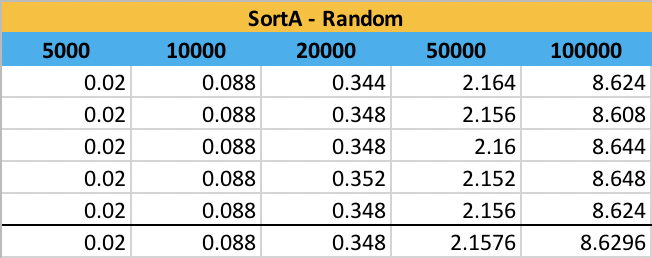
\includegraphics[width=\linewidth]{A_R.png}
	\end{center}
	\end{figure}
\pagebreak
	\begin{figure}[h!]
	\begin{center}
	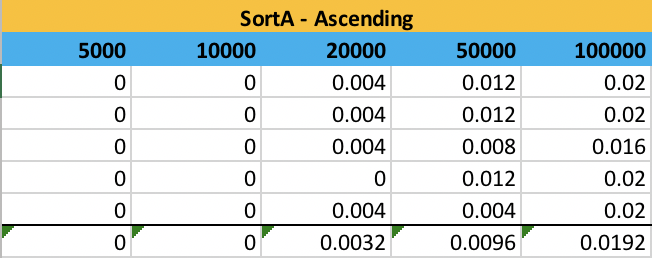
\includegraphics[width=\linewidth]{A_S.png}
	\end{center}
	\end{figure}

	\begin{figure}[h!]
	\begin{center}
	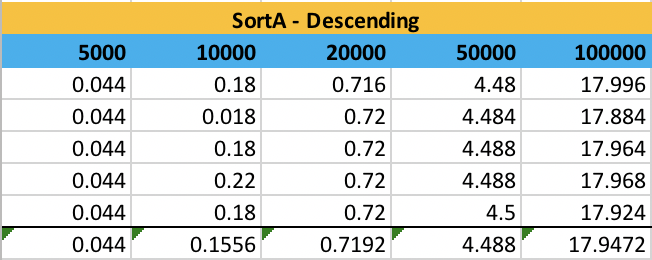
\includegraphics[width=\linewidth]{A_Re.png}
	\end{center}
	\end{figure}

	\begin{figure}[h!]
	\begin{center}
	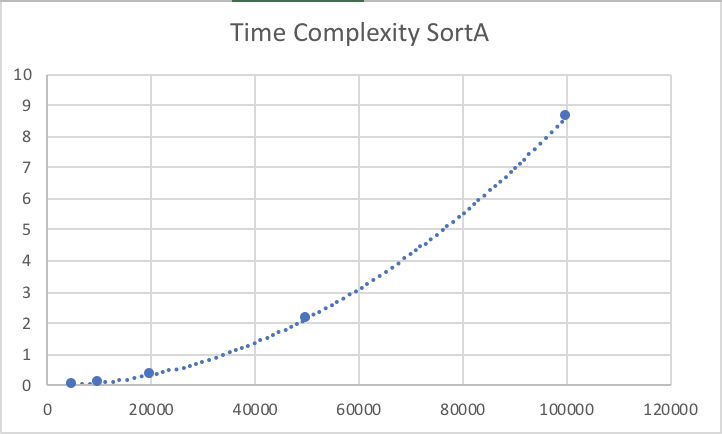
\includegraphics[width=\linewidth]{A_TC.png}
	\end{center}
	\end{figure}
	\pagebreak

\subsection{Program B}

	\begin{figure}[h!]
	\begin{center}
	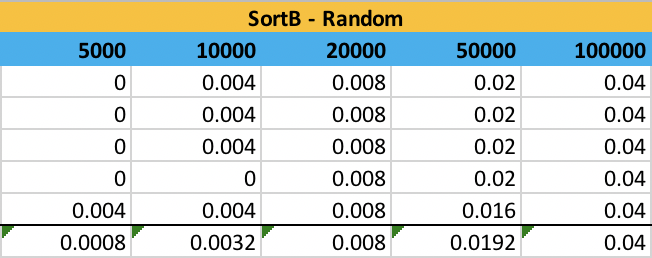
\includegraphics[width=\linewidth]{B_R.png}
	\end{center}
	\end{figure}

	\begin{figure}[h!]
	\begin{center}
	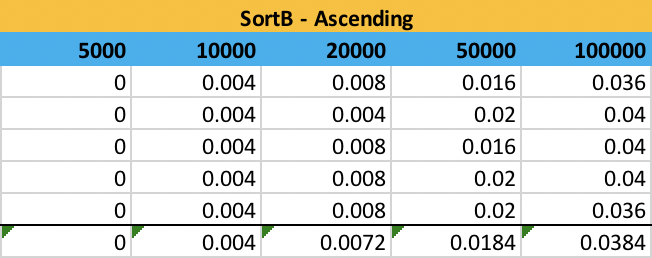
\includegraphics[width=\linewidth]{B_S.png}
	\end{center}
	\end{figure}

	\begin{figure}[h!]
	\begin{center}
	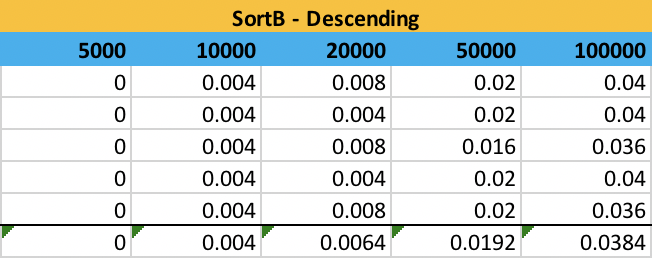
\includegraphics[width=\linewidth]{B_Re.png}
	\end{center}
	\end{figure}

	\begin{figure}[h!]
	\begin{center}
	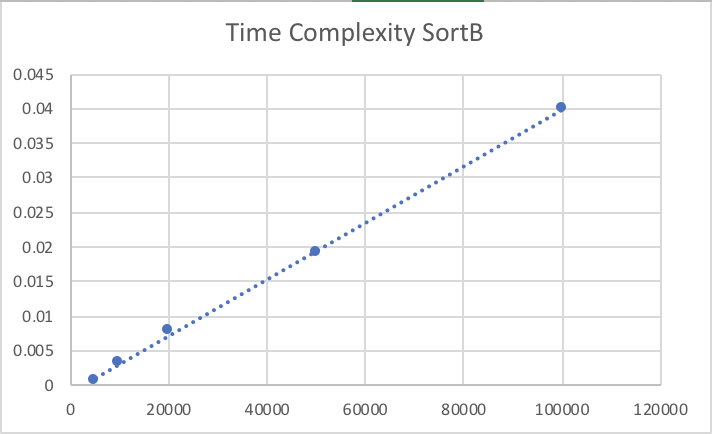
\includegraphics[width=\linewidth]{B_TC.png}
	\end{center}
	\end{figure}





\end{appendices}

\end{document}